\documentclass{beamer}

\mode<presentation>
{
  \usetheme{CambridgeUS}      % or try Darmstadt, Madrid, ...
  \usecolortheme{default} % or try albatross, beaver, crane, ...
  \usefonttheme{default}  % or try serif, structurebold, ...
  \setbeamertemplate{navigation symbols}{}
  \setbeamertemplate{caption}[numbered]
} 

\usepackage[english]{babel}
\usepackage[utf8x]{inputenc}
\usepackage{listings}
\usepackage[ampersand]{easylist}



\definecolor{KTI_green}{RGB}{150, 189, 13}
\definecolor{TU_red}{RGB}{255, 55, 81}
\definecolor{faint_gray}{RGB}{180, 180, 180}

\definecolor{syntax_green}{rgb}{0,0.6,0}
\definecolor{syntax_gray}{rgb}{0.9, 0.9, 0.9}
\definecolor{syntax_mauve}{rgb}{0.58,0,0.82}

\lstset{ 
  backgroundcolor=\color{syntax_gray},  % choose the background color
  basicstyle=\scriptsize\ttfamily,        		% size of fonts used for the code
  breaklines=false,                		% automatic line breaking only at whitespace
  captionpos=b,                    		% sets the caption-position to bottom
  commentstyle=\color{syntax_green},    % comment style
  escapeinside={\%*}{*)},          		% if you want to add LaTeX within your code
  keywordstyle=\color{blue},       		% keyword style
  stringstyle=\color{syntax_mauve},     % string literal style
  columns=fullflexible,
  frame=single,
  framesep=0.5cm,
  framexleftmargin=0.5cm,
  xleftmargin=0.5cm,
  framexrightmargin=0.5cm,
  xrightmargin=0.5cm,
  frame=tb,                 
    numbers=left,                    
    numbersep=15pt,  
  }
  
  
\newcommand{\logopython}{\raggedleft 
\includegraphics[height=0.5cm]{logo_python}\hspace{0.1cm}\\\raggedright}
\newcommand{\logopythonbottom}{\raggedleft\vspace{-0.8cm}
\includegraphics[height=0.5cm]{logo_python}\hspace*{0.05cm}\\\raggedright}

\title[BSP16 - Inversionsmethode]{Inversionsmethode}
\author{Dickbauer Y., Moser P., Perner M.}
\institute{PS Computergestützte Modellierung, WS 2016/17}
%\date{Date of Presentation}

\begin{document}

\begin{frame}
  \titlepage
\end{frame}

% Uncomment these lines for an automatically generated outline.
\begin{frame}{Outline}
  \tableofcontents
\end{frame}

\section{Aufgabenstellung}
\begin{frame}{Aufgabenstellung}
Erzeugen Sie mit Hilfe der Inversionsmethode N Zufallszahlen f¨ur die Zufallsverteilung
X, die durch ihre Verteilungsfunktion F(x) gegeben ist:
\begin{equation}
   f(x) =
   \begin{cases}
     0 & \text{für } x < 0 \\
     1 - \frac{1}{1+x^2} & \text{für } x \geq 0 \\
   \end{cases}
\end{equation}
\begin{itemize}
  \item Eingabe: Anzahl an Zufallszahlen
  \item Output: Zufallszahlen
\end{itemize}

\end{frame}

\begin{frame}{Grafische Darstellung der Funktion}
	\centering
  	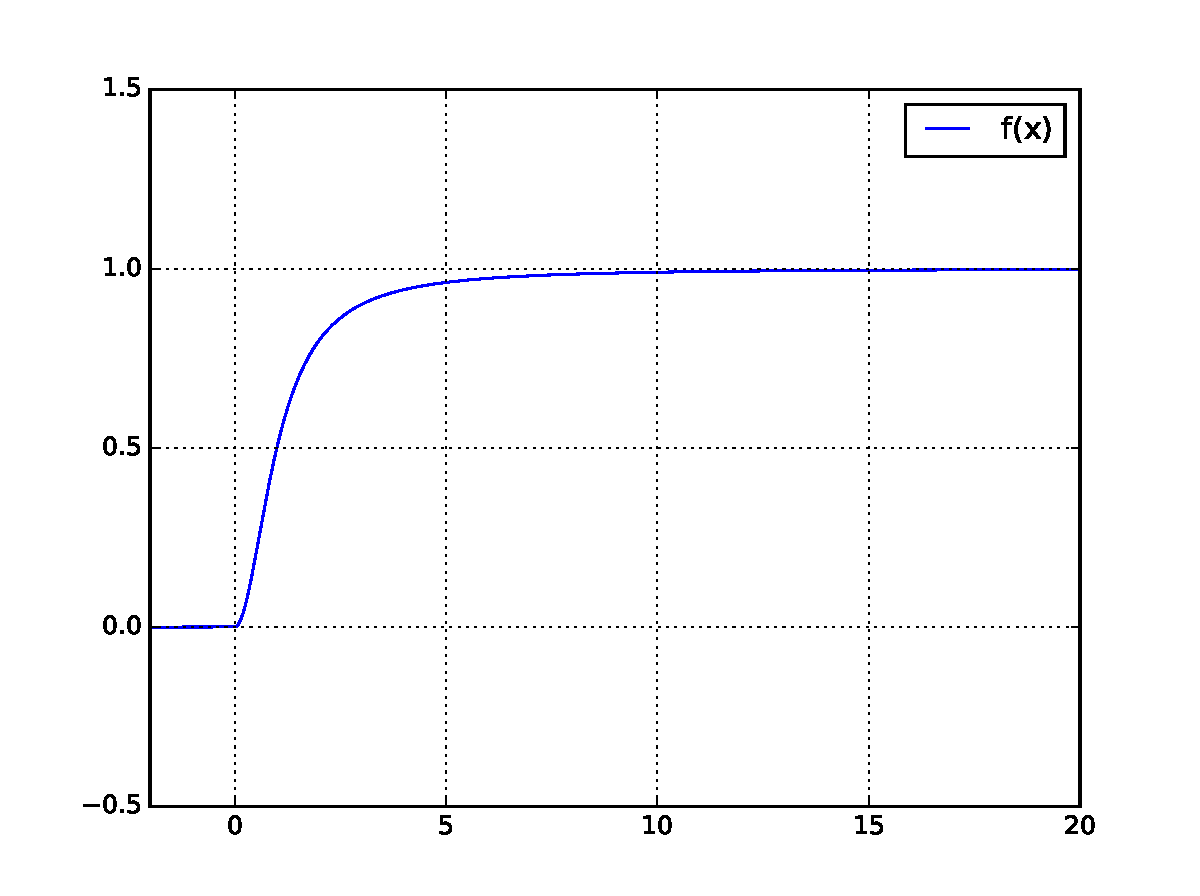
\includegraphics[scale=0.5]{BSP16_plot_function.pdf}
\end{frame} 

\begin{frame}{Inversionsmethode}
\begin{equation}
   f(x) =
   \begin{cases}
     0 & \text{für } x < 0 \\
     1 - \frac{1}{1+x^2} & \text{für } x \geq 0 \\
   \end{cases}
\end{equation}
\begin{equation}
   f^{-1}(x) =
   \begin{cases}
     0 & \text{für } x = 0 \\
     \pm \sqrt{\frac{1}{1-x} - 1} & \text{für } 0 > x < 1 \\
   \end{cases}
\end{equation}
	\centering
  	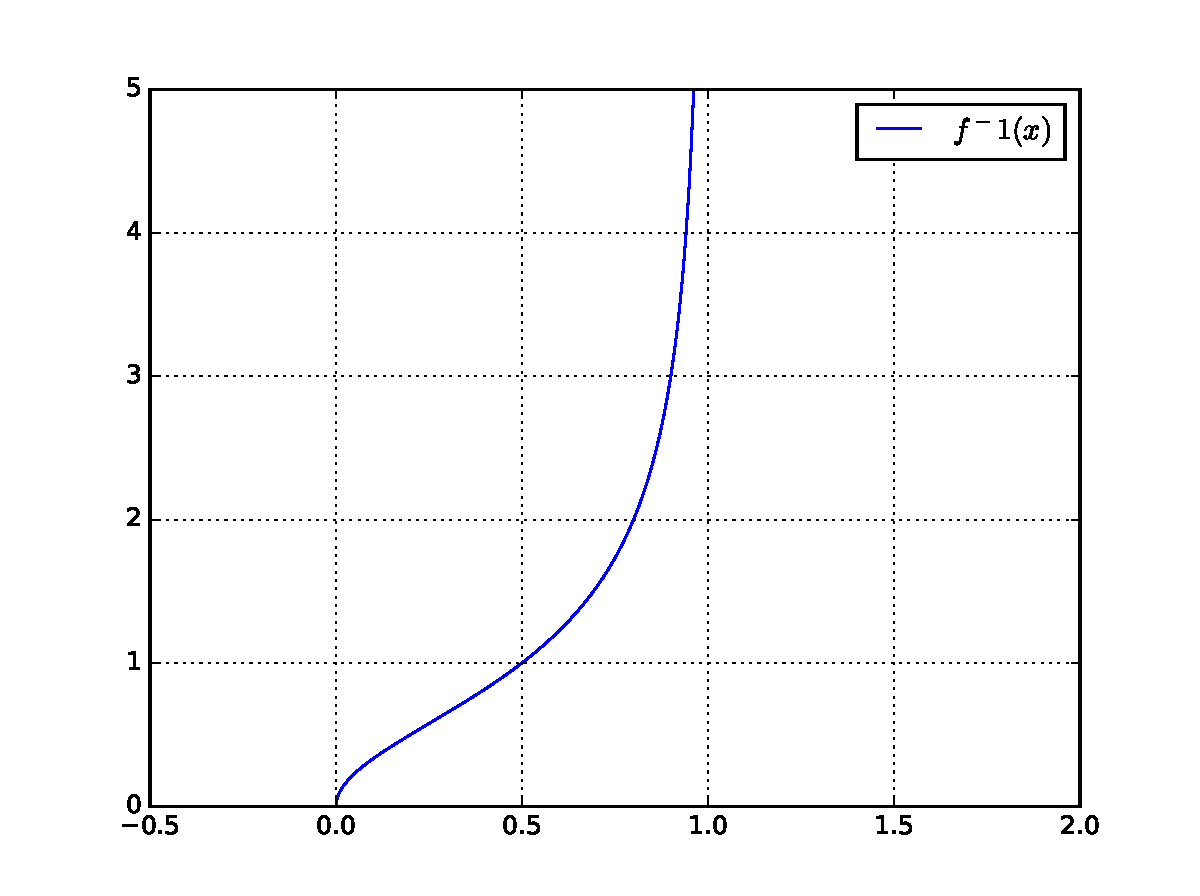
\includegraphics[scale=0.3]{BSP16_plot_function_inverse.pdf}
\end{frame}

\section{Flow Chart}
\begin{frame}{Flow Chart}
	\centering
  	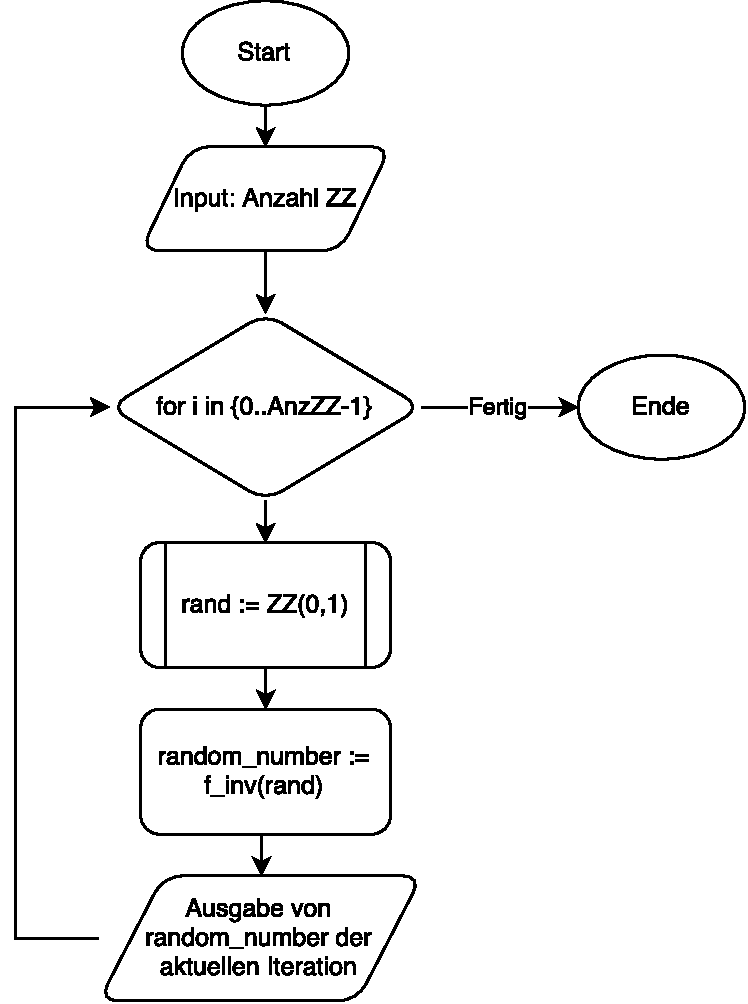
\includegraphics[scale=0.4]{BSP16_FlowChart.pdf}
\end{frame}

\end{document}
